\chapter{Návrh softwarového řešení}
Pro softwarové řešení byla provedena základní analýza požadavků na systém, ze které se specifikovaly funkční a nefunkční požadavky. Na základě těchto požadavků bylo rozhodnuto o zvolených technologiích a architektuře softwaru.
\section{Analýza požadavků na systém}
Diagram užití, který je ztvárněn na obrázku, \ref{fig:usecase} je pro uživatele velice jednoduchý, protože aplikace má být intuitivní a slouží pouze k jednomu účelu a to zadání nové analýzy dat. Pro vývojáře bude nabízet možností více a to zejména ladění algoritmů.

\begin{figure}[h]
	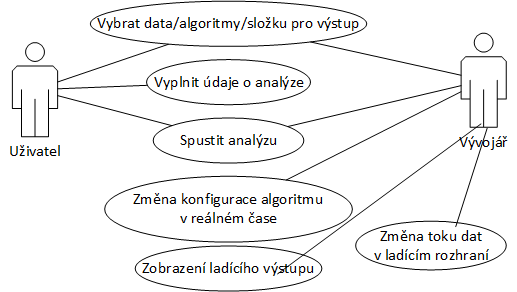
\includegraphics[scale=1]{usecase}
	\centering
	\caption{Diagram užití \label{fig:usecase}}
\end{figure} 

\subsection{Funkční požadavky}

\begin{table}[h]
	\centering
	\begin{tabular}{|
			>{}l |l|}
		\hline
		\multicolumn{1}{|c|}{\bf Funkční požadavek} & \multicolumn{1}{c|}{\bf Popis} \\ \hline
		\begin{tabular}[c]{@{}l@{}}Vybrání dat/algoritmů/\\ složky pro výstup\end{tabular} & \begin{tabular}[c]{@{}l@{}}Aplikace zobrazí dialog pro výběr dat, \\ algoritmů a složky pro výstup.\end{tabular} \\ \hline
		Vyplnění údajů o analýze & \begin{tabular}[c]{@{}l@{}}Aplikace nabídne formulář pro vyplnění\\ názvu a popisu analýzy.\end{tabular} \\ \hline
		Spuštění analýzy & Aplikace spustí analýzu dat. \\ \hline
		\begin{tabular}[c]{@{}l@{}}Změna konfigurace algoritmu\\ v reálném čase\end{tabular} & \begin{tabular}[c]{@{}l@{}}Aplikace umožní změnu konfigurace\\ algoritmů v reálném čase pro lepší\\ ladění algoritmů.\end{tabular} \\ \hline
		Zobrazení ladícího výstupu & \begin{tabular}[c]{@{}l@{}}Aplikace zobrazí ladící výstup aktuálně\\ zpracovávaného snímku, jako nové okno\\ s obrázkem snímku.\end{tabular} \\ \hline
		\begin{tabular}[c]{@{}l@{}}Změna toku dat v ladícím\\ rozhraní\end{tabular} & \begin{tabular}[c]{@{}l@{}}Aplikace umožní vývojářům přehrávat\\ již analyzované video, posouvat rychlost\\ přehrávání či vybrat konkrétní snímek.\end{tabular} \\ \hline
	\end{tabular}
	\caption{Funkční požadavky na aplikaci}
	\label{tab:funkcni}
\end{table}
\FloatBarrier
\subsection{Nefunkční požadavky}

\begin{table}[h]
	\centering
\begin{tabular}{|
		>{}l |l|}
	\hline
	\multicolumn{1}{|c|}{\bf Nefunkční požadavek} & \multicolumn{1}{c|}{\bf Popis} \\ \hline
	Intuitivní ovládání & \begin{tabular}[c]{@{}l@{}}Aplikace bude jednoduchá k použití\\ i bez manuálu.\end{tabular} \\ \hline
	Optimalizace & \begin{tabular}[c]{@{}l@{}}Aplikace musí zvládat zpracovávat\\ velké množství dat a být co\\ nejefektivnější.\end{tabular} \\ \hline
	Generování výstupních souborů & \begin{tabular}[c]{@{}l@{}}Aplikace bude umět generovat výstup\\ do předem zvolených formátů.\end{tabular} \\ \hline
	Multiplatformní použití & \begin{tabular}[c]{@{}l@{}}Aplikace by měla být nezávislá na \\ konkrétní platformě.\end{tabular} \\ \hline
\end{tabular}
\end{table}
\FloatBarrier

\begin{table}[h]
	\centering
	\begin{tabular}{|
			>{}l |l|}
		\hline
	Možnost implementace více GUI & \begin{tabular}[c]{@{}l@{}}Aplikace by měla být navržena tak, aby\\ bylo možné vystavět na ní různá rozhraní\\ např. desktop nebo web.\end{tabular} \\ \hline
	Oddělené prostředí & \begin{tabular}[c]{@{}l@{}}Vývojové prostředí bude oddělené od\\ produkčního, aby zbytečně nedocházelo k\\ nepředvídatelným chybám. Bude pouze\\ využívat část společné funkcionality.\end{tabular} \\ \hline
\end{tabular}
	\caption{Nefunkční požadavky na aplikaci}
	\label{tab:nefunkcni}
\end{table}


\section{Použité technologie a knihovny}
Tato kapitola se zabývá použitými technologiemi a knihovnami. Technologie byly zvoleny na základě autorových zkušeností s nimi a také vhodností pro charakter práce. Následující výčet ukazuje hlavní technologie použité v práci, mimo ně jsou ještě použity různé podpůrné knihovny od Apache, které již však nejsou klíčové pro funkčnost a spíše usnadňují práci.
\begin{itemize}
	\item Java - objektově orientovaný programovací jazyk vyvinutý společností Sun Microsystems a později odkoupen společností Oracle. Java je multiplatformní jazyk, tudíž není problém spustit jeden kód na více operačních systémech či zařízení. V práci je použita Java 1.8\_0.45 a je tak minimální podporovanou verzí pro spuštění software. V práci jsou využity nejmodernější přístupy, které Java 1.8 přináší.
	\item JavaFX8 - technologie pro tvorbu bohatých klientských aplikací. Je jednou z možných implementací \gls{glos:GUI} aplikace (více o \gls{glos:GUI} v kapitole \ref{sec:arch}). Od verze Javy 1.8 je již standardem pro tvorbu \gls{glos:GUI} a nahrazuje starý swing.
	\item OpenCv - knihovna pro počítačové vidění pod licencí BSD. Knihovna nabízí mnoho nástrojů pro práci s obrazovými daty a je vysoce optimalizovaná pro produkční aplikace. Využívá nativní kód přímo pro určité platformy a hardwarovou akceleraci pomocí OpenCL, pokud je možná. Je hlavním nástrojem pro výpočty a manipulaci s obrazem, v Jave jsou napsány pouze minoritní výpočetní operace\cite{learning}
	\item Apache Maven - nástroj pro sestavování programu, řešení automatických závislostí na knihovny a správy modulů projektu.\cite{maven}
	\item Apachae POI - knihovna pro manipulaci různých formátů založených na Office Open XML standars a Microsoft OLE 2 Compound Document format. Lze tak vytvářet a pracovat se soubory XLS a XLSX, případně číst další soubory vytvořené z Microsoft Office.\cite{apache-1}
	\item Apache PDFBox - knihovna, která umožňuje vytvářet PDF dokumenty, manipulovat s existujícími a získávat obsah dokumentů.\cite{apache-2}
	\item ProGuard - nástroj, který minimalizuje, optimalizuje, obfuskuje a před ověřuje Java třídy. Umí detekovat a odstranit nepoužívané třídy, pole, metody a atributy pro zmenšení výsledného kódu. Optimalizuje bytecode a odstraňuje nepoužívané instrukce. Přejmenovává zbývající třídy, pole a metody použitím krátkých nevýznamných jmen, aby nebylo jednoduché program dekompilovat. Přeznačuje a před ověřuje existující třídy pro Java 6 a vyšší, aby tak zrychlil jejich načítání.\cite{proguard} V práci je použit jako plugin do Mavenu při sestavování programu.
	\item Launch4J - nástroj pro obalování spustitelného Java programu nativním kódem pro Windows a vytváření tak .exe souborů. Nástroj také umožňuje definování minimálního JRE a případě přesměrování na stránky pro stažení případně je možné vložit celé JRE, jako knihovnu, kterou nástroj bude načítat pří spuštění programu.\cite{launch4j} V práci je použit jako plugin do Mavenu při sestavování programu.
\end{itemize}

\section{Vývoj algoritmů}
K zjištění přítomnosti krve v trávícím traktu nebylo možné použít stejné principy pro všechny možné případy výskytů krvavých oblastí. Proto byly vyvinuty dva algoritmy pro detekci velkých a malých skvrn, které používají víceméně stejné metody, ale odlišné postupy. Jediná stejná část pro oba dva algoritmy je, že se na začátku zpracování ořízne obraz kvůli vznikajícím barevným anomáliím na okrajích snímací části kamery.
Popis algoritmů je zde obecný bez použití konkrétních nakonfigurovaných hodnot, v příloze \ref{sec:prilohaKonfig} a \ref{sec:prilohaHodnoty} jsou vidět konkrétní hodnoty a jejich vysvětlení.
\subsection{Detekce malých skvrn}
Algoritmus je rozdělen na dvě nezávislé částí, které se pak na konci porovnají, a v případě schody se snímek vyhodnotí pozitivně.

První část je zaměřena na filtrování obrazu dle určitého barevného rozmezí, která je zpřesněna dalšími technikami.
\begin{enumerate}
	\item Převod barevného formátu z BGR do HSV. S HSV formátem je možné přesněji vyjádřit barevné rozmezí, které je potřeba zachovat, viz obr. \ref{fig:alg_1}.E.
	\item Filtrace matice dle definovaného barevného rozmezí. Výsledkem operace je nová matice, která obsahuje pouze vybrané barvy a jejich hodnoty jsou reprezentovány jako binární data, dochází tedy ke ztrátě barevné informace, viz obr. \ref{fig:alg_1}.F.
	\item Pro všechny spojité oblasti, které vznikly z předchozího kroku, se vypočte jejich oblast a ponechají se pouze ty, které jsou větší než definovaná hodnota. Tím dojde k odstranění nevýznamných miniaturních oblastí, které jsou pravděpodobně vzniklé šumem, případě jinými anomáliemi. A také se vyplní nevybarvené oblasti uvnitř spojitých oblastí, viz obr. \ref{fig:alg_1}.G.
	\item Na všechny body s hodnotou 1 ve vyfiltrované matici se zkopíruje barevná informace z původní HSV matice, tím se vrátí barevná informace k dalšímu zpracování, viz obr. \ref{fig:alg_1}.H.
	\item Provede se morfologická operace dilatace dle zadané konfigurace. Tím dojde ke spojení všech blízkých bodů v matici a vzniknou tak větší spojité oblasti, kde by potencionálně mohla být krev, viz obr. \ref{fig:alg_1}.I.
	\item Pro všechny spojité oblasti, které vzniknou po dilataci, se vypočte jejich ohraničující čtverec, který se vyřízne z matice.
	\item V každém takto vzniklém čtverci se provede znovu filtrování dle barvy, ale s jinou "přisnější" konfigurací. V nově vzniklé matici už se nefiltrují malé artefakty a provede se rovnou dilatace. To má za následek, že se v podstatě nic nezmění, nebo se čtverec rozpadne na více oblastí, anebo dojde k vyřazení čtverce z potencionálních detekovaných oblastí.
	\item V každém takto upraveném čtverci se najdou všechny spojité oblasti, ohraničí se čtvercem a uloží se do pole, které v sobě drží ostatní \gls{glos:ROI}, viz obr. \ref{fig:alg_1}.J.
\end{enumerate}

\begin{figure}[h]
	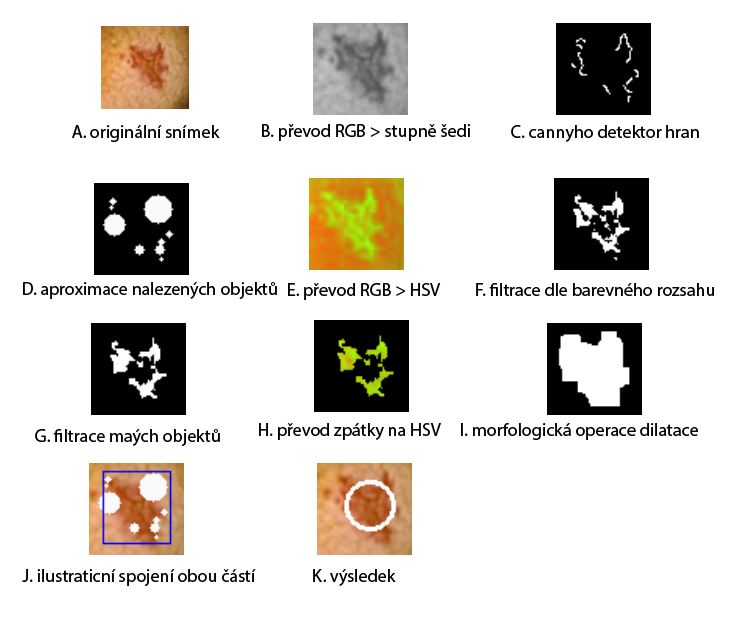
\includegraphics[scale=0.5]{alg1}
	\centering
	\caption{Ukázka průchodu algoritmu detekce malých skvrn. \label{fig:alg_1}}
\end{figure} 
\FloatBarrier

V druhé části algoritmu se detekují hrany a určí se tak potencionální objekty, které jsou odlišné od pozadí. Postup je následující:
\begin{enumerate}
	\item Převod barevného formátu z GRB na odstíny šedi, jelikož je k detekci hran vhodnější, viz. obr. \ref{fig:alg_1}.B.
	\item Gaussovo rozmazání dle definované konfigurace.
	\item Cannyho detektor hran dle definované konfigurace, viz. obr. \ref{fig:alg_1}.C.
	\item Pro všechny spojité nalezené hrany se vypočte minimální obklopující kružnice. Ta slouží, jako jednoduchá aproximace hledaného objektu.
	\item Jelikož vznikají anomálie při detekci hran a zejména okrajové části kamery jsou často zahrnuty ve výsledku, tak je nutné vybrat pouze ty kružnice, které nepřesahují maximálně definovaný průměr. Je v podstatě nemožné, aby se tímto odstranila hrana, která se nemá odstranit, protože tento algoritmus detekuje pouze menší skvrny a anomálie, které vznikají jsou velmi velké.
	\item Zanesení zbylých kružnic do pomocné matice, viz. obr. \ref{fig:alg_1}.D.
\end{enumerate}

Jakmile jsou k dispozici obě části algoritmu, tedy matice, která obsahuje pomocné kružnice, a list všech \gls{glos:ROI}. Tak dojde k vyhodnocení, zda-li je matice pozitivní. To je provedeno iterací přes všechny čtverce v listu a pokud se v oblasti konkrétního čtverce nachází alespoň jeden bod z kružnice, tak je místo pozitivní, viz obr. \ref{fig:alg_1}.K.


\begin{figure}[h]
	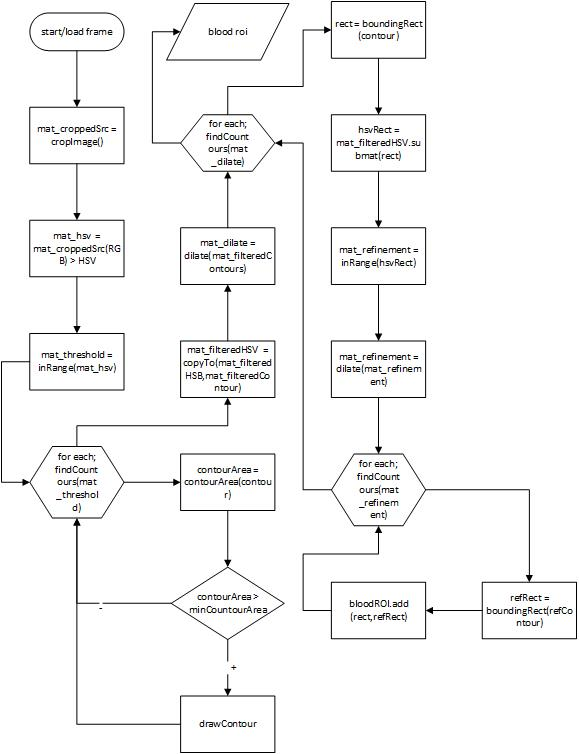
\includegraphics[scale=1]{sb_diagram_1}
	\centering
	\caption{Vývojový diagram první části algoritmu detekce malých skvrn. \label{fig:sb_diagram_1}}
\end{figure} 
\FloatBarrier

\begin{figure}[h]
	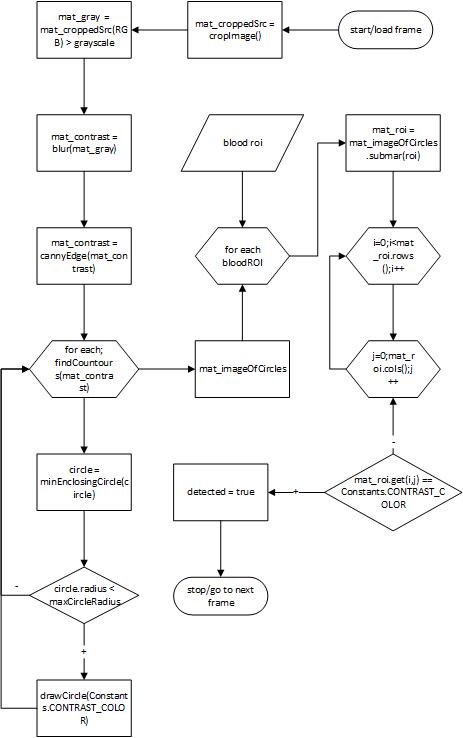
\includegraphics[scale=1]{sb_diagram_2}
	\centering
	\caption{Vývojový diagram druhé části algoritmu detekce malých skvrn a spojení obou částí. \label{fig:sb_diagram_2}}
\end{figure} 
\FloatBarrier


\subsection{Detekce velkých skvrn}
Konstrukce druhého algoritmu je značně jednodušší a přímočařejší než-li detekce menších skvrn. Jedná se o nalezení velké oblasti se stejným barevným spektrem. Postup je následující:

\begin{enumerate}
	\item Převod barevného formátu z BGR do HSV, viz obr. \ref{fig:alg_2}.B.
	\item Filtrace matice dle definovaného barevného rozmezí, viz obr. \ref{fig:alg_2}.C.
	\item Filtrování miniaturních částí, viz obr. \ref{fig:alg_2}.D.
	\item Morfologická operace dilatace, viz obr. \ref{fig:alg_2}.E.
	\item Pro všechny spojité oblasti v matici se zjistí jejich plocha. Ta se porovná proti definované procentuální velikosti celkové oblasti a pokud je větší, tak se rámec vyhodnotí pozitivně. Např. pokud je spojitá oblast větší než-li 15\% celkové oblasti, viz obr. \ref{fig:alg_2}.F.
\end{enumerate} 

\begin{figure}[h]
	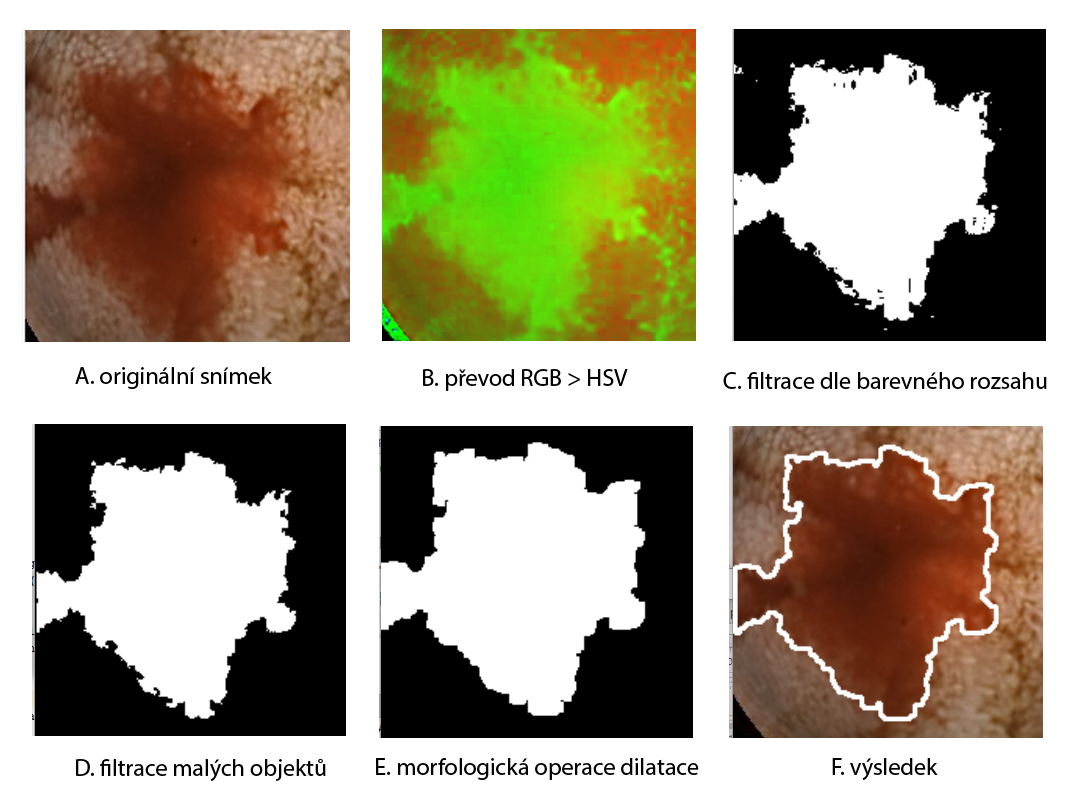
\includegraphics[scale=0.3]{alg2}
	\centering
	\caption{Ukázka průchodu algoritmu detekce velkých skvrn. \label{fig:alg_2}}
\end{figure} 


\begin{figure}[h]
	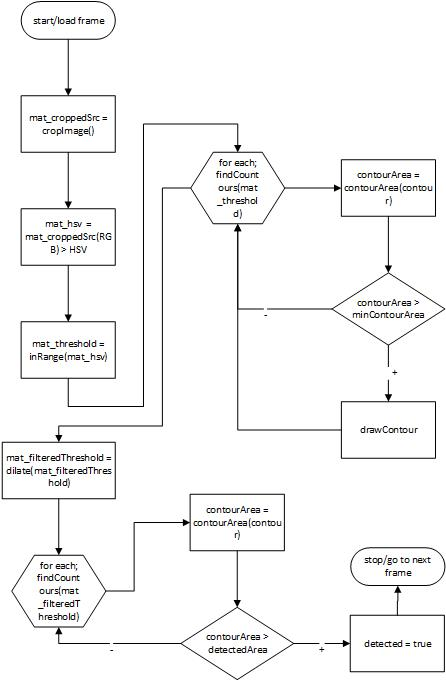
\includegraphics[scale=1]{bb_diagram}
	\centering
	\caption{Vývojový diagram algoritmu velkých skvrn. \label{fig:bb_diagram}}
\end{figure} 